\section{Policy Building}
\label{sec:design_pol_build}

The most complex aspect of using the \theResServer system for a user is the creation of policies for resources that the user wants to encrypt \& upload. For example, a user does not necessarily know all the attributes that have been signed into user keys (since they are extensible) and even if they have access to a list of attributes, they may not know which values are valid for a given attribute.

Since we cannot expect a user to read the formal language definition for \thePolicyLang (\Cref{sec:formal_lang}), as it is a technical definition, we need to provide a tool for a user to build policies with. This tool needs to inform the user of all presently assigned attributes and the possible values an attribute may accept, ensuring a consistent \& compatible use of attributes across all policies. The tool needs to enforce correct types on the values the user inputs and generate a \thePolicyLang policy from the inputs, which is then interpreted to a \PyOpenABE-compatible policy.

\begin{figure}[htp]
    \centering
    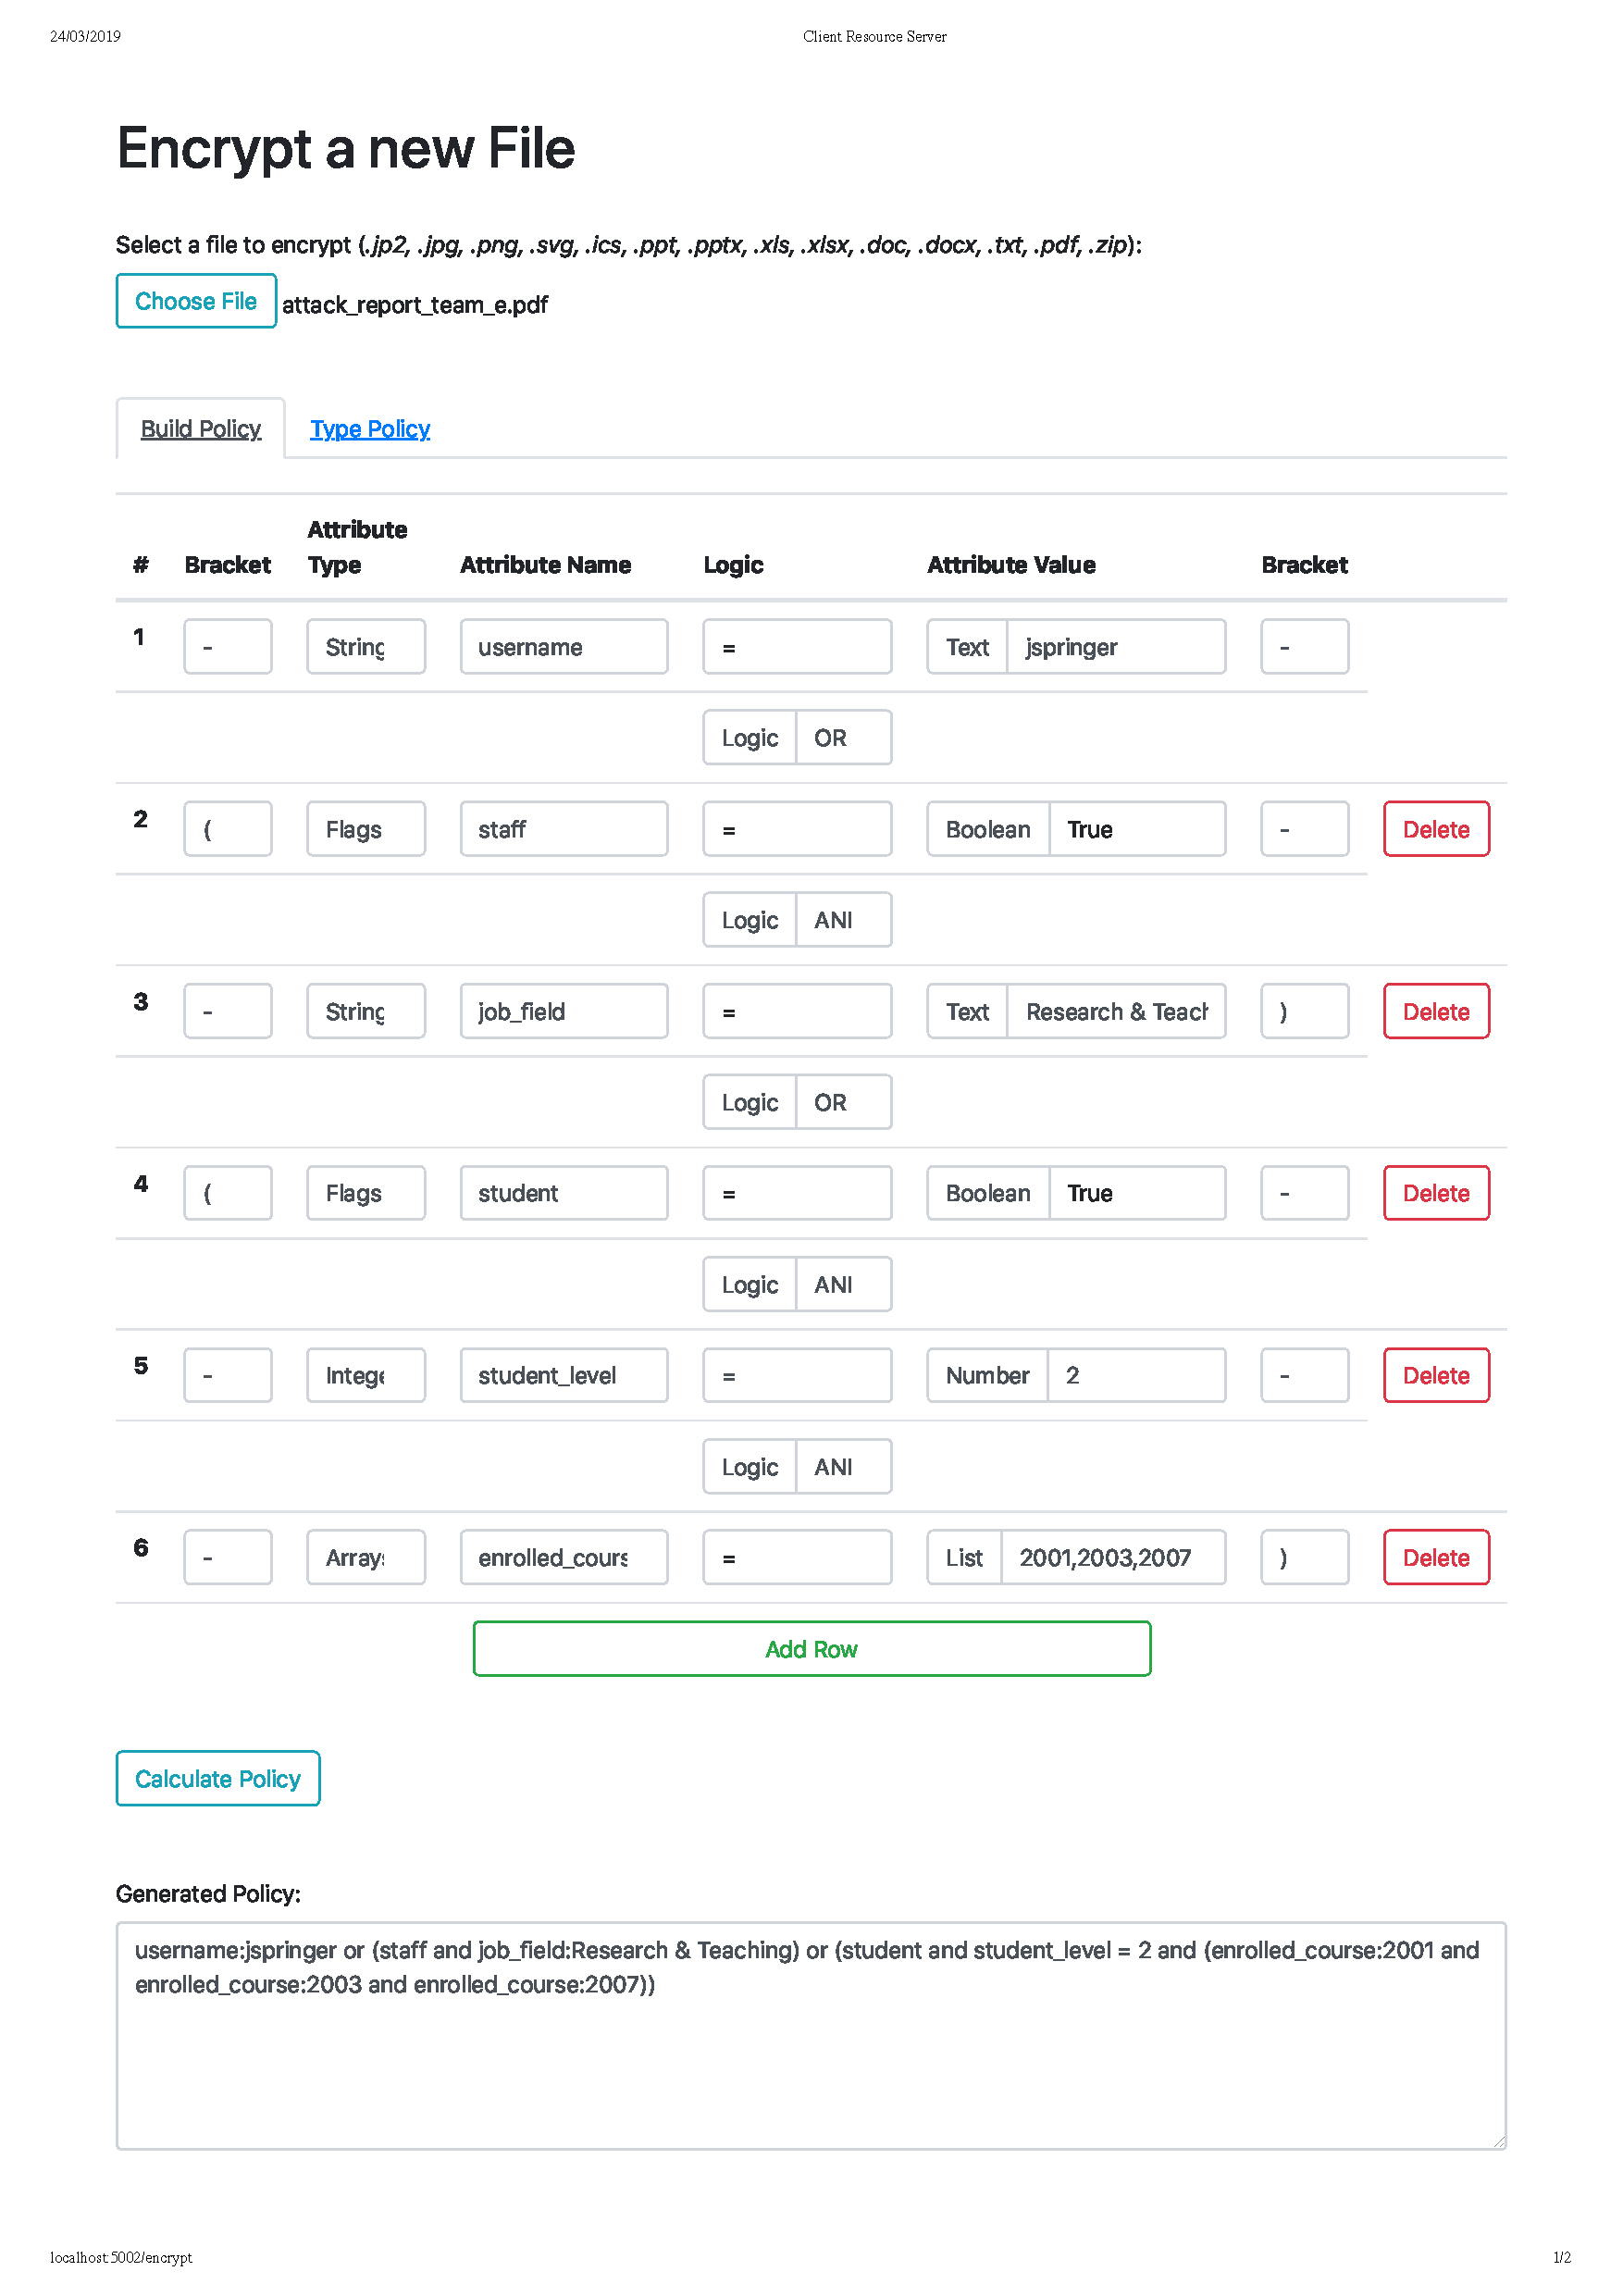
\includegraphics[width=\linewidth,keepaspectratio]{appendices/building_policy.pdf}

    \caption{
      \label{fig:policy_builder}
      Screenshot of the Build Policy tool in the Client Resource Server simulating the creation of the policy required for Case Study \#1, \Cref{fig:case_study_policy_1}.
    }

\end{figure}

\Cref{fig:policy_builder} presents a screenshot of the resulting \acrshort{html}-based policy builder, as implemented for the \acrfull{crs}, and specifically shows the result of building the policy required for Case Study \#1 (\Cref{fig:case_study_policy_1}). The tool allows the user to build the policy line-by-line using dropdown fields that are pre-populated with the current attributes in use by the \theResServer system, which are collected, periodically from the \acrshort{prs}. The \acrshort{prs} in turn, receives them from the \acrshort{mks} via offline updates by \acrshort{dcs} Admins staff members.

Per attribute selected by the user, a \acrshort{html} input field is created that enforces the type for the value the user must input via \acrshort{html}5 form validation \citep{Foundation2019}. The user can then `calculate' the resulting policy and a \PyOpenABE compliant policy is returned in textbox for the user to verify. If the policy is as expected, the user can continue with encrypting their desired file, again using the \acrshort{crs} with the \PyOpenABE library of bindings.
